% // final project report / paper

\documentclass{acm_proc_article-sp}
\usepackage{natbib}
\usepackage{algpseudocode}

\begin{document}

\title{Making Ant Colony Optimization Parallel}
%\subtitle{[Extended Abstract]

\numberofauthors{3} 

\author{
\alignauthor
Doug Patti\\
       \email{pattid2@rpi.edu}
% 2nd. author
\alignauthor
Ziv Kennan\\
       \email{kennaz@rpi.edu}
% 3rd. author
\alignauthor Patrick Phipps\\
       \email{phippp@rpi.edu}
}

\maketitle
\begin{abstract}

This paper provides a look into the thought processes, considerations, results and
implementation details of our final project: parallelizing the ant colony 
optimization to solve the traveling salesman problem within a reasonable bound. 

It then provides a discussion on the results of the modified algorithm,
comparing it to a serial solution as well as studying the scaling properties
on two different computer systems. The two systems used in this study will be
an optimized high perfomance system called Kratos and a Blue Gene/L system here
at RPI.

\end{abstract}

\terms{Traveling Salesman Problem}

\keywords{Parallel, MPI, Ant Colony, Optimization, TSP}

\section{Introduction}
Computationally hard problems commonly come up when attempting to solve
useful and practical problems. One such problem is the traveling salesman 
problem. This is a well known problem in the computer science community. Formulated
in 1930 \citep{graphtheory} this problem is heavily studied as a case of an optimization problem.
The premise of the problem is thus: given a list of cities and the distances
between them pick a shortest path that visits each of them exactly once and
returns to the starting city. 

We chose to use the ant colony optimization to solve this problem. The ant colony
technique is a probalistic technique that relies on sending out many ants that
all take random paths, the best path is chosen and is more emphasized for
the next iteration of ants. Over time this will converge to the best
solution found. This technique was first discussed by Marco Dorigo in \citep{optimization} for his
PhD thesis. His application was similar to the one we have chosen but the technique
has been applied to other NP-Hard problems.

\section{Serial ACO Algorithm}
All ACO algorithms begin with a graph. To begin the algorithm, an ant is placed on each node of the graph.
At each iteraion of the algorithmm every ant chooses a new node to go to. It does this based on a probabilistic 
schema. Each edge has two weights. The first weight is proportional to the distance between two cities. The second
weight is fundamental to the ACO scheme, it is the pheromone weight. The ant picks an edge based on a random roll
relative to these two weights. These ant choosing iterations are repeated until the ants have completed a full tour
of the graph. 

Upon all the ants completing a full tour of the graph the ant with the shortest tour is picked and a global decay is
applied to all the edges' pheromone weights. The algorithm then takes the best ant's tour and adds to the relevant 
edge's pheromone weight accumulator. The purpose of this step is to emphasis this edge in future ant walks. The algorithm
is repeated until the ants begin to converge on a result. 

\caption{Serial ACO}
\begin{algorithmic}[1]
    \Procedure{ACO}{$g}\Comment{Returns best path in g}
        \State $ants$ \Comment{Array of ants} 
        \While{not converged}
            \ForAll{$ants \to ant$} 
                \State $ ant.tour $
            \EndFor
            \State $ decay\ all\ pheromone\ trails $
            \State $ find\ best\ ant\ trail $
            \State $ increment\ all\ edges on\ best\ trail $
        \EndWhile
    \EndProcedure
\end{algorithmic}

\section{Parallel ACO Algorithm}
There are several modifications that are necessary to transform serial ACO to parallel ACO. The first task
necessary in parallelizing ACO is the partitioning of the graph. This can be done in a variety of ways but 
this step is considered pre-processing as it makes sense to process a potentially large graph once and load it
from the disk when it's needed. Potential partioning schemes include: round robin, clusters distribution, 
random distribution among other methods.

For our inital implementation, we chose a round robin graph partitioning scheme since it was relatively easy to implement
and worked well with our implicit graph representation, which uses a hash function to calculate and store distances between
nodes. Clustering schemes are perhaps better suited to this application since they can reduce the amount of network traffic,
and speed up the time needed to find a solution.

After partitioning the graph, the ACO algorith is run on each node. During each iteration an ant attempts to make a tour. 
However, it will inevitably find that it needs to visit a node that is absent from the processor responsible for it. 
At this point, the ant is sent over to the proper processor. Once it is received there, it joins the rest of the ants
on that processor in the queue waiting its turn to process. After being sent around to every processor at least once, visiting
all of the nodes in the graph, the ant has completed its tour. The processors then do a reduce in themselvesto see what ant(s)
had the best tour. A reduction is then done over all processors that sums the total number of ants that have shortest tours.
Every processor then expects to receive that many ants minus the number of shortest tour ants that it currently has. This is the
sync step, now all processors have a copy of the best tour ants. Each processor then updates the pheromone weights using 
the best ants' tours. 

A somewhat trivial improvement to this algorithm that cannot be done on the Blue Gene is to have threads process the ants in the queue.
This can be somewhat tricky to implement with all of the coordination that must go on in order to keep the processes from having
unexpected behavior. 

\caption{Parallel ACO}
\begin{algorithmic}[1]

    \Procedure{ACO}{$g}\Comment{Returns best path in g}
        \State $ants$\Comment{Array of ants}
        \While{not converged}
            
            \While{every ant has not visited my nodes}
            
                \ForAll{$ants \to ant$} 
                    \State $ ant.tour $
                \EndFor
                
                \State $receive\ new\ ants $
                \State $add\ new\ ants\ to\ ants\ queue $
            
            \EndWhile
            
                \State $perform\ reduction\ to\ determine\ smallest\ tour $
                \State $count = reduction\ sum\ of\ total\ smallest\ tour\ ants $
                
                \If{$I\ have\ a\ smallest\ tour\ ant$}
                    \State $send\ ant\ to\ all $
                \EndIf
                \State $ receive\ (\ count\ -\ my\ smallest\ tour\ count\ )\ ants $
                \State $ decay\ all\ pheromone\ trails $
                \State $ find\ best\ ant\ trail $
                \State $ increment\ all\ edges\ on\ best\ trail $
    
        \EndWhile
    \EndProcedure
    
    \Procedure{Ant Tour}{$ant$}\Comment{Parallel Ant Tour}
        \While{$ all\ nodes\ not\ visited$}      
            \State $Determine\ edge$
            \If{$edge\ is\ not\ on\ processor$}
                \State $send\ ant\ to\ processor\ with\ edge$
                \State $break$
            \EndIf
            \State $Take\ edge$
        \EndWhile
    \EndProcedure
    
\end{algorithmic}

\section{Implementation Details}
Our implementation is in C/MPI, with a preliminary version by Doug in python as a test of the ACO algorithm. A custom hash and queue are both used as a basis for most of the ACO implementation, with mpi serving to synchronize nodes. mpi allreduce is used heavily to find the best pheremone levels and tours across all nodes at the end of each iteration, and non-blocking sends and recieves are used to send ants between nodes and for all other communications. 

\section{Testing and Results}
We ran a battery of testing configurations on both Kratos and the IBM Blue Gene L at the CCNI. To get a wide survey of our algorithm's performance we tested all three graph partitioning methods on Kratos. Taking the best
performing method and using that to test on the Blue Gene in order to alleviate the potential of running over the 10 minute execution time limit. On Kratos we ran a graph of 4,096 nodes on 5 different 
processor configurations: 1, 2, 4, 8, and 16. We ran these runs using each of our three partioning schemes: round robin, distance, and clustering. We then took the best perfoming method out of these tests
and ran an 8,192 node graph using all of the above listed processor configurations. An important note to our results is that Kratos is time to complete 10 iterations of our algorithm. On the Blue Gene we timed only one iteration to ensure that we could run the largest processor counts as well as the smallest processor counts in the limit. The results of these runs are present in the graphs below.

\begin{figure}[h!]
    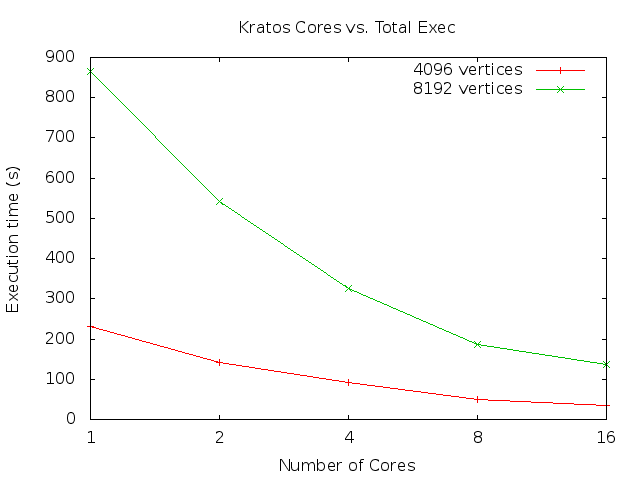
\includegraphics[scale=0.38]{kratostotalexec.png}
    \caption{Total Execution Time vs. Core Count on Kratos using distance partioning}
\end{figure}

\begin{figure}[h!]
    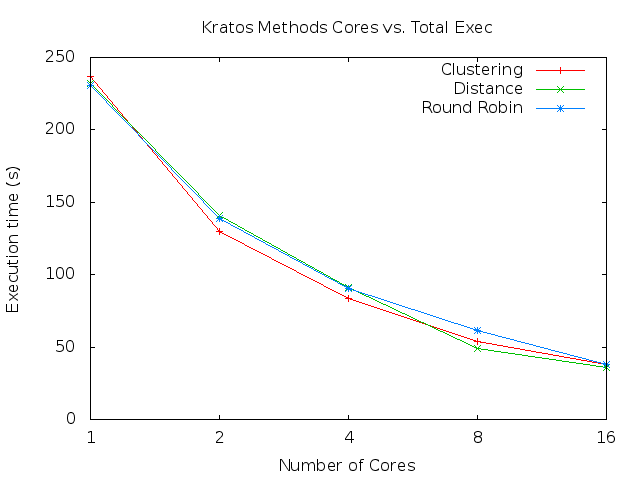
\includegraphics[scale=0.38]{kratosmethods.png}
    \caption{Total Execution Time vs. Method/Cores on Kratos on 4,096 nodes}
\end{figure}

Taking a closer look at the Kratos results we can see that our implementation exhibits strong scaling qualities. For case of 4,096 nodes vs. execution time (red line) it is shown that for a problem of this size
the algorithm gets faster as more cores are added, but it is not a very dramatic improvement. As we scale up the problem size to 8,192 the scaling properties of our algorithm begin to show through. From the serial
version of almost 900 seconds is cut to less than 200 seconds using 16 cores. The trend of this line exhibits the excellent time reductions given by additional processors. With the scaling propertiees of the algorithm
being demonstrated in the first graph, the second shows demonstrates the difference made by using other partioning techniques. In general we see that the round robin partioning scheme yields the worst performance. The
cause of this is the number of times ants have to cross cores. With the round robin scheme there is no sense of order to the nodes in each processor, thus each ant has a higher probability of needing to be 
transfered on its next move. The clustering scheme works well for relatively small core counts but is beat out in the end by the distance method. However, it is interesting to note that on the graph size of 4,096 all
three methods give competitive times for the 16 core case. Further testing on larger graph sizes is required to really see how these partioning schemes affect performance.

\begin{figure}[h!]
    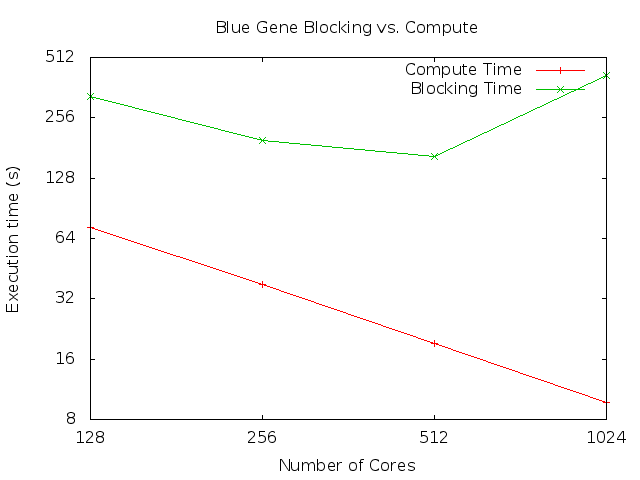
\includegraphics[scale=0.38]{bgtransfercompute.png}
    \caption{Blue Gene Blocking Time vs. Computation Time}
\end{figure}

\begin{figure}[h!]
    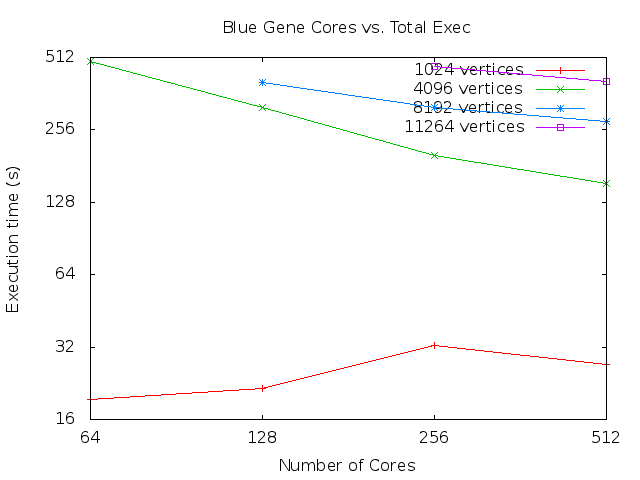
\includegraphics[scale=0.38]{bgtotalexec.png}
    \caption{Blue Gene Total Execution time vs. Core Count - various graph sizes}
\end{figure}

We see in the computation time vs. transfer time (message passing time) that transfer time is clearly the bottleneck in the performance of our algorithm. These Blue Gene results utilize the clustering partioning method.
The rational behind using this method is that it performed best on Kratos, and that we want to choose the method with the overall lesser amount of ant transfers on average which the distance method delivers. As expected
the time spent computing drops linearly with the amount of cores, as the amount of processing done relative to transfers as the core count increases becomes small. Looking at the total execution time vs. cores for various
problem sizes on the Blue Gene it is important to note that the TODO VIRTUAL MODE DISCUSSION

An interesting observation of the tests that we ran is that the Blue Gene is out performed by Kratos for the problem sizes that we used. The assumption being that we did not achieve proper graph size to core count
ratios to maximize the Blue Gene, implying that there is an optimization problem to maximize the algorithm in the problem size to core ratio. It is also important to realize that we are not saturating Kratos' bandwidth
in sending ants across the network, meaning that processor speed is more important in the test battery that we used in testing than the speed of the network.

\section{Comparison to Serial ACO TSP}
Our algorithm is written such that it takes advantage of n cores, from 1 to k, where k is the maximum number of cores available to the system. Large problem sizes will have difficulty fitting on a single core's
worth of memory. Our algorithm is intended to require less memory per processor as the number of processors increases, so the more processors you have the bigger the problem size you can handle even if each processor
has a relatively small amount of memory. From the graphs above, we can see that the parallelized version was successful at least as far as outperforming its serial competitor; the parallel version being
roughly 7 times faster on the largest test case that was run on Kratos. 

\section{Conclusions}
The Ant Colony Optimization problem sets out to solve an NP-hard problem, giving little hope to a well scaling serial solution. We set out to adapt this algorithm to the parallel programming domain by splitting up the graph problem into process sized chunks. By spliting up the graph we necessarily complicate the problem slightly by requiring a communication scheme that allows us to maintain an ant taking a complete tour across the graph by moving between the processes. It is also required that we can sync the best trail across all of the partial graphs. 

We believe that we have met the requirements that we had set forth for ourselves on this project, and while we never got to attempt to see how our algorithm works on our theoretical Blue Gene memory limit of around 120,000 nodes the tests performed gave us a good idea of how well our implementation actually works. We have seen from the results sections that on the whole the algorithm had more impressive completion times on Kratos and that our
scaling properties were very well pronounced on that system. The results we have obtained from the Blue Gene show a general trend of improvement as the core count increased we speculate that the problem sizes tested 
were not properly scaled to the processor counts we had accesss to.


\section{Future Work}
The first avenue of future work for this project is to more thoroughly test our implementation. Ideally, we would acquire more processing time on the Blue Gene and work out some discrepencies we had been observing in
VN mode runs vs. non-VN mode runs with VN mode hindering algorithm performance. With the 700mHz processors in the Blue Gene we cannot get through one iteration of problem sizes > 18k nodes in 10 minutes. These larger problem
runs can give us better insight as to how the algorithm performs on the Blue Gene as a whole, considering that our smaller problem size results were better overall on Kratos we would like to scale out to problems
that could not fit on Kratos.

While our implementation and exploration are relatively robust and thorough, there are many ways in
which this project could be further improved and explored. One option that might provide an easy performance
boost is to use threading (pthreads) in addition to MPI. While we didn't have time to explore this, it is a relatively
straightforward extension, and on a hardware-threaded system such as BG/Q it might provide significant
performance boosts.

Another interesting extension to our work is to use genetic algorithms in addition to ACO to further 
increase the quality of our solution while also allowing the algorithms to run in fewer iterations. Genetic
algorithms can be usaed to generate string mutations which iteratively create better routes for the ants to follow,
instead of choosing random routes to start off with.

One of the limitations of our implementation is that we use a round-robin distribution on an implicitly defined graph; 
this means that not only can an arbitrary explicit graph not be used with our system, but any graph used is not partitioned
in an optimal manner. As mentioned above, alternative partitioning schemes and support for explicit graphs are two important features that we would add to our system in the future.

One of the last improvements we would like to make to our implementatino is the ability to auto tune certain internal parameters
of the algorithm based on the quality of the solution desired and the speed at which it is needed. By adjusting the step and decay functions for our pheremone levels (alpha, beta, etc) as well as adjusting the precision of the numbers we use we can greatly affect the runtime performance of our implementation. Since we ran into some issues using floats, we switched to doubles early on, but that decision could be made at runtime depending on the type of solution desired. By auto-tuning all of these parameters our implementation would have much more flexibility; however given the time-frame we had, we were unable to do this.

\section{Acknowledgments}
We would like to thank professor Carrothers for the feedback he provided to 
our group during the project, as well as the tips he gave us throughout the
semester, they were very helpful in completing this project.

\section{Work Distributionn}
The idea was chosen by all three group members collaboratively, and fleshed out 
during a group meeting. Most of the coding was done with all three members present,
with Doug writing most of the code and other members providing input and aiding with
debugging. The paper was written by all three group members collaboratively, with Ziv
and Patrick doing most of the actual writing. Each step of the algorithm was written out
in comments in the source files to be filled out later. All group members participated in this
pseudo-coding step of our process. 


\bibliographystyle{plain}
\bibliography{references}

\balancecolumns

\end{document}
